\section{Use Case} 
\label{sec:usecase}

We have been working closely with scientists at the Argonne Advanced Photon Source (APS) to understand their current applications and workflows that would need an integrated research infrastructure including edge and high-performance computing to fully utilize next-generation X-ray beamline facilities. After a series of discussions with the scientists, we identified some user applications as future workloads and recognized their requirements for running them across the continuum (see Fig.~\ref{fig:use-case}.) 
In this section we use a specific use case of X-ray imaging to explain the need for a computing continuum.

\subsection{Background}

The Argonne APS user facility provides ultrabright, high-energy X-ray beams to
scientists to serve scientific experiments ranging from materials science to
biology, chemistry, planetary science, and fundamental physics. The facility is
now finalizing its recent upgrade~\cite{apsupgrade} and raises the need for
data transportation and storage for their next-generation X-ray beams and
state-of-the-art detectors. Advancing from manual data aggregation and processing,
the APS facility is designed to stream data within a centralized computing
architecture and control system, linked with HPC systems. Terabytes of data per
experiment are automatically sent to HPC data storage and are consumed by
scientific simulations running on HPC. With the APS upgrade, scientists expect
10--1000x data volume increase toward petabytes per experiment. Such an increase
in data volume demands the advancement of data aggregation and processing
capabilities within the edge-to-HPC computing continuum. The introduction of computation within and at
the edge in combination with HPC brings \textit{new opportunities and
challenges} in expanding the computing continuum and AI-driven control in the
new APS operation. 

%Additionally, the Atmospheric Radiation Measurement~\cite{arm} research facility utilizes distributed instrumentation to gather long-term Earth science data for studying atmospheric phenomena and climate patterns including the Energy Exascale Earth System Model~\cite{e3sm}.
%
%Beyond these research facilities, researchers distributed sensor networks to study other domain sciences, such as renewable energy sources~\cite{boyson2007performance}, watersheds~\cite{fox2022sulfur}, and wildfires~\cite{dewangan2022figlib}.


%Advancing from manual data aggregation and processing, the APS facility is designed to stream data within a centralized computing architecture and control system, linked with HPC systems. Terabytes of data per experiment are automatically sent to HPC data storage and are consumed by scientific simulations running on HPC. Note that in the post APS upgrade scientists expect 10-1000x data volume increase towards Petabytes per experiment.

In addition to the high-bandwidth computing and networking systems in the infrastructure, ML-based AI methods at the edge (built, trained, and validated on HPC) will enable scientists to analyze data directly at the edge. Recent AI-based applications~\cite{babu2022deep, Cherukara:2020il, liu2020braggnn} and dynamic workflows~\cite{kandel2023demonstration} have been proposed and developed by APS scientists. These AI techniques are now commonly employed by experimental scientists, running on hardware-accelerated machines for data analysis, often surpassing the performance of traditional numerical computing methods, particularly for feature detection and image reconstruction, such as finding and tracking Bragg peaks and ptychography. 

Within the continuum, AI@Edge models can be dynamically reconfigured and play active roles in driving the dynamic adaptation of the scientific instruments to react to changes in experimental conditions. We believe that this new computing paradigm will continue to evolve and will require an integrated end-to-end system to manage resources across scientific workflows. In order to support these new functionalities, fine-grained resource management will need to administer shared computational and storage resources at the edge, while the connections to HPC resources and workflow management will need further improvements. To co-design such an integrated system, we discuss here a recently started project, named Charon, that explores the design space of system software for connecting and adapting resource-constrained AI@Edge workloads to HPC, through fine-grained resource management.

%The introduction of computation within and at the edges in combination with HPC brings \textit{new opportunities and challenges} in expanding the computing continuum and AI-driven control in APS operation. This edge-to-HPC continuum will make it possible to analyze data at the edge including the use of machine learning (ML)-based artificial intelligence (AI), which are built, trained, and validated on HPC, depending on the capabilities of the edge computing machine. Moreover, the AI at the edge (``AI@Edge'') models can be dynamically reconfigured and can play active roles in driving the dynamic adaptation of the scientific instruments to react to changes in experimental configurations. In order to support these new functionalities, fine-grained resource management to administrate shared computational and storage resources at the edge is required, and its connection to HPC resource and workflow management needs to be designed. 

% raises three new capabilities that have the potential to transform the relationship between experimental and computational science. 


%% AI at the Edge
% First, data analysis at the edge has become a reality, including the use of machine learning (ML) based artificial intelligence (AI) depending on the capabilities of the edge computing machine. Waggle~\cite{beckman2016waggle} edge computing platform already supports diverse AI-driven data analysis at the edge (``AI@Edge''). The instruments provide not only timely data streams for the data storage at HPC and AI models at the edge but also interfaces to \emph{steer the experiment}.

%% reconfiguration
%Second, AI at the edge can be dynamically reconfigured and can play active roles in driving the dynamic adaptation of the instruments. Given the computational requirements of training ML model, the update of ML models activity is best performed by integrating edge and HPC systems. Harnessing the continuum will enable HPC applications to be effectively extended beyond just analyzing data, becoming an integral part of user facilities, providing on-the-fly optimizations of AI@Edge codes for the instruments.
%Such performance requirements will demand a robust, common middleware and operating system (OS) layer spanning the continuum, dynamically adapting edge computing to \emph{improve on performance of facilities and instruments and the efficacy of scientific experiments}.

%% resource management
% Third, edge computing in an IRI will support many disparate and simultaneous workloads, which will compete for limited edge resources requiring arbitration. Early use of edge scheduling capabilities in Waggle, which provides a multi-tenant edge scheduler to manage multiple science users sharing nodes and running codes at the edge~\cite{kim2022goal}, reveals the need for much finer-grained resource management in order to administrate shared computational and storage resources on the scale envisioned.

% TODO1: merge the 3 paragraphs into the 2nd paragraph --  Done (SP)
% TODO2: Talk about the APS problem and how we can solve this 


%Recent AI-based applications~\cite{babu2022deep, Cherukara:2020il, liu2020braggnn} and dynamic workflow~\cite{kandel2023demonstration} that were proposed and developed by APS scientists, have changed their traditional computing requirements to support the new workloads. These AI techniques are now commonly employed by experimental scientists and running on hardware-accelerated machines for data analysis, particularly feature detection and image reconstruction, often surpassing the performance of traditional numerical computing methods. We believe that this new computing paradigm will constantly evolve and impact the current computing continuum and will require an integrated end-to-end system to manage resources across the computing continuum. To co-design such an integrated system with the new paradigm in the domain science, we present here Charon, a project to explore the design space of system software to connect and adapt resource-constrained AI@Edge workloads to HPC, in terms of fine-grained resource management.

%In the following sections we introduce a target use case requiring resource management and arbitration across the computing continuum for a scientific workflow. We then detail our methods and experimental setup and summarize our approach and future direction.

% These opportunities and challenges motivate us to explore the design space of system software to connect and adapt resource-constrained AI@Edge workloads to HPC. Specifically, we will investigate: 1) how resource constraints on edge devices can be alleviated by dynamically adapting the edge environment, arbitrating resources to ensure the necessary performance for experiment-critical applications while enabling additional uses for the edge, 2) how system software can help design AI@Edge applications that leverage HPC platforms to tune their models and redeploy improved models on the fly, and 3) how flexible the user-agnostic system software policies can be, in order to be deployed across a wide range of use cases and hardware setups.

%Given the short timeframe of this proposal, the team intends to leverage existing software and collaborations across Argonne, allowing us to quickly prototype and validate our approach and identify unknowns and future priority research directions for system software in the computing continuum.

% We draw on two scientific use cases where connecting AI@Edge to HPC will be beneficial: real-time analysis with beamline detectors and distributed environmental sensing.  These vastly different use cases---one a scientific user facility and the other  a geographically distributed network---will help guide our design.

\begin{figure}[tb]
  \centering
    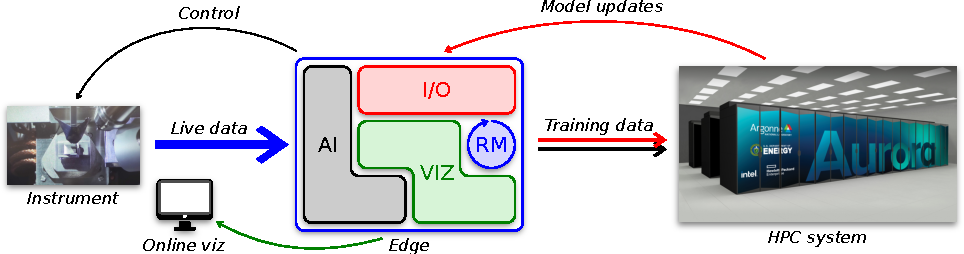
\includegraphics[width=1\linewidth]{figures/aps-use-case.pdf}
  \caption{Our main use case: an AI@Edge model controls the scientific instrument and processes live data while being periodically updated based on fine-tuning and retraining taking place on HPC resources.}
  \label{fig:use-case}
\end{figure}


% \paragraph{Real-Time Beamline Data Processing}
% (see Fig.~\ref{fig:use-case})
% context: APS-U + Waggle Spring 2023 example
% figure from paper with AI updates
% description of the full use-case:
%  - detector connected to edge via network
%  - edge running AI inference (image reconstruction)
%  - control based on AI inference
%  - data processing for storage and fine tuning
%  - AI model updates computed on HPC
% Goal: demonstrate (in simulation) the full pipeline, using existing tech
% Resource Arbitration: constraints and adapting to workload performance





% Despite the fact that a variety of scientific applications requiring remote sensing and real-time analysis can benefit from this end-to-end integrated infrastructure, we initially focus on a scientific application from APS scientists that urgently needs such an infrastructure to fully utilize their next-generation X-ray beams~\cite{apsupgrade}. After a series of discussions with the scientists, we recognize the following user applications as future workloads running across the continuum (see Fig. \ref{fig:use-case}.)

\subsection{Core Capabilities in Edge-to-HPC}


% \textcolor{blue}{Reviewer1: From the description of figure 1, it is unclear why this use-case needs a computing continuum. It looks like a set of services deployed at the edge connected to a HPC back-end. It could be defined as a Cyber-Physical System composed of actuators, sensors, edge devices and an HPC back-end. What is the architecture and design of the foreseen computing continuum here?}

% \textcolor{blue}{(Response: We highlight the need of a computing continuum in the user case in the ``Core Capabilities in edge-to-HPC'' section.)}

%\paragraph{\textbf{AI/ML-Based X-ray Image Reconstruction}}
%
%The recognized AI-based method processes a raw X-ray scan and reconstructs an image from the scan; this 3 MB tiny model~\cite{babu2022deep} can take various resolutions (64x64--128x128) and run in parallel to match with detector's sampling speed, fr example,  2 kHz. A single instance of the current implementation performs at approximately 100 Hz on an N

%\paragraph{\textbf{AI Model Retraining at HPC}}
%\paragraph{\textbf{Timely AI Model Retraining at HPC}}
\textbf{Timely AI Model Retraining on HPC}
%
An example of AI-based data processing is image reconstruction from raw X-ray diffraction patterns using small but powerful convolutional neural networks~\cite{babu2022deep}. Fine-tuning and retraining of the neural network per experiment with various input sizes on an HPC system can adapt the model to new measurements during a beamline experiment~\cite{babu2022deep}. A newly obtained dataset from the edge must arrive at the HPC resource, and model retraining must be scheduled in a timely manner, in order to update the model.
%that is now fine-tuned for the current experiment running at the edge.
Anomalies in the data stream can also be identified and extracted by data processing at the edge and selectively added to the dataset, since they might be new patterns that the AI model needs to learn in HPC.

% \textcolor{red}{does that create a need for data selection at the edge? if so, we could hint at more data processing at the edge for this, as well as model update}

%To retrain and fine-tune a ptychography model, for example, a full diffraction pattern from beams of incident X-rays in diverse directions are required to provide a variety of patterns and features that makes the model reconstruct images more accurately.


%\paragraph{\textbf{Real-Time Sensor Reconfiguration and Control}}
\textbf{Real-Time Sensor Reconfiguration and Control}
%
X-ray diffraction patterns are collected
%Samples are exposed to an X-ray beam 
in different positions and angles by moving the sample mount during the experiment for X-ray ptychography and crystallography. Scientists run programs to operate actuators and change the configuration of sensors and the experiment environment (e.g., pressure, temperature). Such actuation and reconfiguration are simple tasks but should be applied immediately and not be interrupted and delayed. Recently, Argonne scientists proposed an AI-enabled workflow to control a detector probe for efficient probe scanning~\cite{kandel2023demonstration} in real time using AI@Edge. This AI-driven decision-making demands high-throughput computation for the model to keep up with the sampling rate of the detector. Scaling AI inference and aggregation of the results require precise resource allocation to support real-time control and prevent bottlenecks. 

%\paragraph{\textbf{Data Reduction On the Fly}}
\textbf{Data Reduction on the Fly}
%
APS scientists estimate that the data volume in the post-upgrade era will increase by orders of magnitude toward petabytes per experiment, making filtering out uninteresting data highly desirable. Performing computations on the live data at the edge not only can reduce the final data volume but also can identify interesting phenomena occurring during the experiment. Filtering conditions vary per experiment: under known conditions, we may further reduce the total data volume, whereas exploratory experiments may need the full stream of data for new discovery. In the end, scientists will receive meta information from the edge computation to efficiently index and search through the reduced data. In addition to the capabilities identified above, we expect other workloads, such as live visualization, local AI fine-tuning at the edge, and caching of raw data to persistent storage, to introduce additional resource constraints to the end-to-end infrastructure.

% Earlier in 2023, the Waggle team explored
% this opportunity by deploying a small set of Waggle nodes near an APS beamline (see Fig.~\ref{fig:waggle-aps}). This collaboration focused on latency-constrained inference, demonstrating that an
% AI@Edge workload yielding timely experimental insight could be of benefit.

%
% Furthermore, nanoscale materials scientists at Argonne recently proposed an AI-enabled workflow to control a detector probe for an efficient probe scanning~\cite{kandel2023demonstration} in real time using AI@Edge. This AI-driven decision making demands high-throughput computation on graphics processing units (GPUs) to keep up with the frame rate of the detector. Scaling AI inference and aggregation of the results require precise resource allocation to support real-time control and prevent bottlenecks. Meanwhile, AI fine-tuning and retraining on an HPC system can adapt the model to new measurements during a beamline experiment~\cite{babu2022deep}.

% Another important aspect to capture in this use case is the data product generation profile to deal with the unprecedented data volume expected after the APS upgrade. Compared to the current data volume manually handled by APS scientists and user community, the data volume in post upgrade era will increase by orders of magnitude toward terabytes per experiment, making filtering out uninteresting data highly desirable. Performing computations on the live data at the edge  not only can reduce the final data volume but  also can identify interesting phenomena occurring during the experiment. 

% Beamline physics is thus an excellent use case to act as our driver: we already have a collaboration with APS to test-deploy Waggle-based AI@Edge resources; and
% live inference, real-time control, and AI-fine-tuning are already identified needs of the post-upgrade APS.

%\kamil{It feels like this whole paragraph (or two?) should be in Research, not Background?}
%To demonstrate the full AI@Edge capability powered by \projectname resource management and monitoring, we will set up an emulation use case mimicking the aforementioned real-world use cases. In our proposed use case, multiple edge devices including Nvidia Jetson and Dell server racks will be connected to a simulated beamline detector. Each edge device running the PtychoNN AI model~\cite{babu2022deep} streams inference results to a data aggregator for visualization and control. Our resource monitoring agent running on each device will measure resource profile of the AI inference as well as system-level metrics such as the network and I/O traffic. We will structure application-level data pipeline using PvaPy~\cite{}, a Python-base tool maintained by APS for data distribution and aggregation. PvaPy makes it possible to probe the pipeline to measure data processing rate at each block to understand application-level performance in the data flow. We will simulate a controller that consumes the AI inference results and controls the simulated detector probe.
% (Yongho) Q: what do we want to control in this use case? How will we create a controller in this use case?

%\paragraph{Multitenancy in Disaster Monitoring at the Edge}
%\swann{paragraph on remote waggle resources being used to monitor several types of weather/disaster events, and the need to arbitrate priorities between the workloads
%associated with it. This is mostly stretch goals, since we don't really have the time to deal with it. It's also helpful to keep in the reviewers mind that it's not just
%resource management of single edge nodes.}

% The increasing size, frequency, and intensity of wildfires --- and their cascading effects on air and water quality as well as on flooding and landslides after subsequent rain events --- are a pressing societal challenge and a complex topic that requires multidisciplinary research.
%
% One of the major underlying problems is a lack of data and verifiable information that results in an insufficient capacity to observe, track, and predict the phenomena that lead to natural disasters in the first place, as well as their devastating secondary impacts.

% In an effort to fill these critical gaps in the available research infrastructure, Waggle edge nodes have been deployed in numerous locations across the United States.
%
% A network of the edge nodes, acting as a core cyberinfrastructure, can provide a standardized, democratic network that makes a range of further scientific inquiries far more feasible, especially in remote areas that might serve as baselines or refuges for organisms that cannot be tracked using GPS.
%
%Spatially extensive yet fine-resolution measurements of physical and
%biological processes, from below-ground to atmospheric, being collected by
%the SAGE sensors, can, e.g., provide critical insight into phenotype
%plasticity and adaptive evolution using newly revealed Rules of Life.  The
%diversity of available sensors can advance convergence research at the
%nexus of public health, environmental inequities, and sources and flows of
%atmospheric and waterborne toxicants.
%
%More generally,
% Real-time and near-real-time sensor networks are considered critical for understanding topics as diverse as the impacts of climate change on the critical zone and the dynamics of volcanic eruptions, reducing the risk and toll of geohazards, and understanding subduction zone processes.

% Given the limited uplink data bandwidth available in many remote areas, it is generally infeasible for Waggle nodes to stream all the collected raw data to a remote data center; the initial data analysis (filtering, identification of potentially interesting phenomena, etc.) must take place at the edge, and these days it is typically AI-driven.  Considering the plethora of potential applications, Waggle edge nodes may host multiple independent application-specific data analysis workloads that could end up competing for node resources; resource arbitration is needed to keep such issues in check.

%Cascading Hazards:  Wildfires, drought, landslides, floods, air and water quality
%The increasing size, frequency, and intensity of wildfires — and their cascading effects on flooding and landslides after subsequent rain events — is one example of a pressing societal challenge and a complex research topic that demands convergent research across biosphere domains. Scientists understand many key relationships among climate, vegetation, and weather that enable extreme wildfires. However, it remains difficult to specifically quantify cascading risks, analyze mitigation impacts, and predict containment challenges for any given year. During events, response is hampered by inadequate forecasts of fire behavior and its implications for suppression and evacuation due to a lack of data, verifiable information, and alert-system efficiency. Following events, there is insufficient capacity to observe, track, and predict the devastating secondary impacts of degraded air and water quality on public health or of extreme weather events that can precipitate landslides and floods. 

%In the absence of real-time, integrative data, predictive models are of little value for informing societal response. In the absence of curated and archived sensor data, some of the longer-term impacts of a changing climate or an environmental hazard become anecdotal.
%SAGE2 will facilitate innovative, hypothesis-driven research on mechanisms by which extreme events and nonstationary climate and other environmental phenomena affect biosphere dynamics that society wishes either to constrain or to conserve. For example, insight into phenotype plasticity and adaptive evolution using newly revealed Rules of Life can emerge from spatially extensive yet fine-resolution measurement of physical and biological processes, from below-ground to atmospheric [16–19].
%Leveraging SAGE as core cyberinfrastructure, SAGE2 will provide a standardized, democratic network to make such inquiries far more feasible, especially in remote areas that might serve as baselines or refugia, and for organisms that must be tracked with radios or chips rather than global positioning system-based transmitters.
%Additionally, the diversity and spatial coverage of sensors supported by SAGE2 will advance Convergence Research at the nexus of public health, environmental inequities, and sources and flows of atmospheric and waterborne toxicants [20–22].

%The U.S. research community has identified sensor networks that are real-time and near-real-time, and that measure across spatial and temporal scales; cyberinfrastructure; and the expertise to use integrated data as priority research capabilities [23–26].
%The NASEM report A Vision for NSF Earth Sciences 2020-2030 cites this need for understanding topics as diverse as the impacts of climate change on the critical zone, the dynamics of volcanic eruptions, how Earth sciences can reduce the risk and toll of geohazards, and understanding subduction zone processes (SZ4D Initiative).
%Similarly, the US Geological Survey natural hazards strategy emphasizes the essential role of multi-sensor networks in mitigating diverse geohazards.
%The NASEM report Climate Change and Ecosystems identified four strategies for advancing the fundamental science that are at the heart of SAGE2: (1) research priorities that include understanding how complexity affects ecological resilience, and identification of early warning metrics and measurements across spatial and temporal scales,
%(2) engagement with diverse audiences, (3) interdisciplinary networks, and (4) translation of science to action.
%SAGE2 will support current and next-generation U.S.-based researchers by filling critical gaps in our nation's research infrastructure. These gaps include poor spatial and temporal resolution of environmental and ecological processes, lack of access to integrative data streams by many of the nation's researchers, and disciplinary silos in sensor science that prevent convergent research. SAGE2 will democratize sensor deployment, support live-streamed data, inform event response capabilities, and facilitate rapid deployment of new technologies, enabling scientists to grow Convergent Research, Harness the Data Revolution, Understand the Rules of Life, and answer key research questions that are responsive to society's urgent needs.
